% Chapter Template

\chapter{Analysis of Fibonacci} % Main chapter title

\label{ChapterX} % Change X to a consecutive number; for referencing this chapter elsewhere, use \ref{ChapterX}


%----------------------------------------------------------------------------------------
%	SECTION 2
%----------------------------------------------------------------------------------------

\section{Introduction}

This chapter analyzes monomial deciders to find a relationship with sequences then attempts to find a law of composition regarding Fibonacci sequences. From the the reinterpretation of the theory, Euler's constant is an example of P = NP because of it's use of calculus. Euler's constant can be defined as 

$\\ $

$e = \sum_{n=0}^{\infty }\frac{1}{n!}$

$\\ $

To show that it is also in the problem set of P $\neq$ NP, start by using the picking function going into infinity. The constant $e$ is the sum of the infinite series of $\frac{1}{n!}$ and can be represented as a series of monomials representing the Decider<x> using the picking function.

$\\ $

$e = (\sum_{n=0}^{\infty }\frac{1}{n!})$

$\\ $

$e = 1 + 1 + 1/(1+1) + 1/(3+3) + 1/(4+(4*3+4*2)+4) + ...$

$\\ $

$e = p_f(Decider<x^0>) + p_f(Decider<x>)+ p_f(Decider<x^2/x> + ...$

\begin{figure}[H]
  \centering
  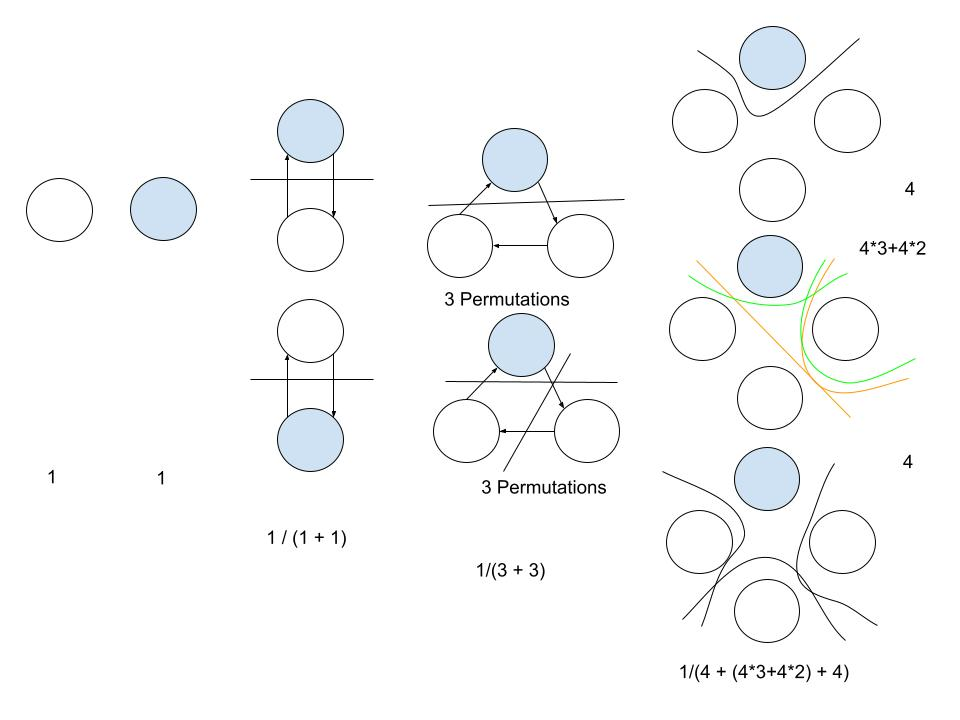
\includegraphics[scale=0.4]{0201Eulers.jpg}
  \caption{Decider that represents the first four terms of the constant $e$.}
  \label{fig:0201Eulers}
\end{figure}



\section{Example of a Decider}

The following is an example of code that roughly sketches a generalized monomial decider, Decider<$2x^2$>. It tests to see if y is in the monomial m(x) = $2x^2$. Although approximation and binary search algorithms work, using this method allows for simplicity of technique in representing a decider visually and gives the reader hands-on potential if they want to experiment on the subject further.

$\\ $

\begin{algorithmic}[1]
\Procedure{GeneralizedDecider}{$y$}
\If {$y = 0$}
     \Return true
\EndIf
\State ($s\gets y$)
\While {$s\geq 0$}
	\For {$i = 0$ to $1$}
		\For {$j = 0$ to $3$}
			\If {$s=0$ and $(j = 0$ or $j = 2)$ and $i = 0$}
				\Return true
			\ElsIf{$s < 0$}
				\Return false				
			\EndIf
			\State $s\gets s - 1$
		\EndFor	
	\EndFor
\EndWhile\\
\Return true
\EndProcedure
\end{algorithmic}

$\\ $

$\textbf{Proof of Correctness}$.

$\\ $

$\textit{Initialization}$. On lines 2 to 3, if y is 0 then it is true. Otherwise, take s to be y.

$\\ $

$\textit{Maintenance}$. The loop invariant starts at line 5 as $s\geq 0$ with value of s being y. While this is true it goes through a for loop on lines 6 to 13 with a starting value of i at 0. At line 7, the last for loop starts with j being a value of 0. On line 8, a condition is checked to see if s is 0, i is 0, and j is either 0 or 2 and returns true if it is. It then passes the for loop with j as the iterating variable until it hits 3 and then the for loop with i as the iterating variable until it hits 1. It continues another pass of the while loop.

$\\ $

$\textit{Termination}$. The while loop on lines 5 to 14 terminate if the for loop on lines 6 to 13 terminate. This for loop terminates if the for loop inside it on lines 7 to 12 terminate. s decreases by 1 on line 11 while once it passes the condition checks and it goes through it at most 2 * 4 times representing the passes in the nested for loop. This algorithm always either returns true or false.

$\\ $

$\textbf{Proof of Time Complexity}$. Starting from the inner most for loop on lines 7 to 12 iterate 3 times. Outside is the for loop on lines 6 to 13 that iterates 2 times. This gives a time complexity of exactly 6 constant. The while loop on lines 5 to 14 has $s\geq 0$ initially s = y which gives a time complexity of $O(y)$. Overall, this gives a time complexity of $O(y+6) = O(y)$. 

$\\ $

$\textbf{Proof of Space Complexity}$. There is only one variable used to keep track of the iteration and that is the variable, s. There are the iteration variables i and j. Hence, the algorithm has a space complexity of a constant, $O(3) = O(1)$.

$\\ $

The above code can be represented visually as follow:

\begin{figure}[H]
  \centering
  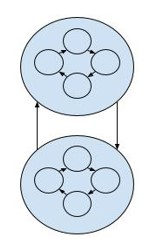
\includegraphics[scale=1]{0202Generalized.jpg}
  \caption{Decider that represents the monomial, $x^3$.}
  \label{fig:0202Generalized}
\end{figure}

\section{Analysis of the Decider $2x^2$}

Data can be extracted to find insight and build a general technique using the generalizedDecider function above for the Decider<$2x^2$>. 


$\\ $

\begin{figure}[H]
  \centering
  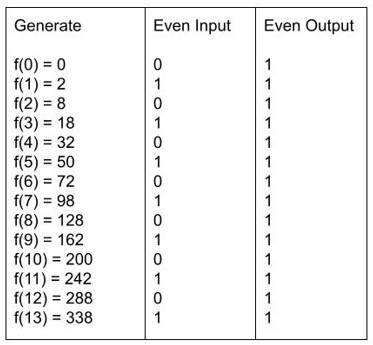
\includegraphics[scale=1]{0203Generate.jpg}
  \caption{Generate function, $2x^2$.}
  \label{fig:0203Generate}
\end{figure}

$\\ $

$\textbf{Generate}$ is f(x) = $2x^2$ = y on the first line and the number of negatives is on the second. There are two finishing and all the even parity outputs end in one state and all the odd parity outputs end on the other. $\textbf{Even Input}$ is the boolean parity of the input being even. $\textbf{Even Output}$ is the boolean parity of the output being odd. 

Here, it can be seen that there is repeating pattern of even and odd values of the following:

$\\ $

$\left[ {\begin{array}{cc}
    1 & 1 \\
    0 & 1 \\
  \end{array} } \right]$

$\\ $

From this array, two finishing states are described. When the input and output are both even and one where the input is odd and the output is even. Every time the head of the tape passes a finishing state, the count of the variable, $\textbf{visit }$is increased by one. Counting the number of visits two the finishing states, it can be seen that for every pair, (start,end), there is a difference of three for $Decider<2x^2>$. The following is a table of the results:

\begin{figure}[H]
  \centering
  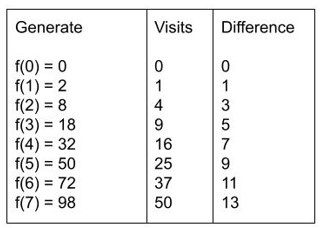
\includegraphics[scale=1]{0204Visits.jpg}
  \caption{Analysis of visits to finishing states in, $2Decider<2x^2>$.}
  \label{fig:0204Visits}
\end{figure}

From analysis, the number of times the tape head visits a finishing state is the difference of the previous input plus two. The difference increases by two every time it passes a finishing state. It doesn't pass when the number of visits is even, so it can be deduced that the difference is increased by two every time it passes the odd finishing state. This result allows us to write a program to decide if y is in $2x^2$.

$\\ $

\begin{algorithmic}[1]
\Procedure{Generator}{$max$}
\State $result\gets [\ ]$
\State $x\gets 0$
\State $difference\gets 0$
\State $i\gets 0$
\While {$x < max + 1$}
	\State $num\gets 2x^2$
	\If {$GeneralizedDecider(i)$}
		\If {$num = i$}
			\State $result[x] = i$
			\State $x\gets x + 1$
			\State $difference\gets 0$
		\Else
			\State $difference\gets difference - 1$
		\EndIf
	\EndIf
	\State $i\gets i + 1$
\EndWhile\\
\Return result
\EndProcedure
\end{algorithmic}

$\\ $

$\textbf{Proof of Correctness}$.

$\\ $

$\textit{Initialization}$. The variables result, x, difference, and i get initiated.

$\\ $

$\textit{Maintenance}$. The loop is invariant with the case $x < max + 1$ which holds true. The $num$ variable is set to $2x^2$. $GeneralizedDecider(i)$ is used to decide if $i$ is in the decider, but it isn't always in $2x^2$. If $num$ is $i$, the variable $x$ is updated to keep the condition of the loop invariant true which is $x < max + 1$. On line 17, the variable $i$ is updated so that on line 8, the condition is always met.

$\\ $

$\textit{Termination}$. Start of with the while loop such that $x < max + 1$. $i$ is incremented every loop so that the condition $GeneralizedDecider(i)$ is always met on line 8. This means that when it visits line 9, the condition is passed and the variable, $x$, is increased moving the while loop on line 6 forward. This allows the algorithm to terminate successfully.

$\\ $

$\textbf{Proof of Time Complexity}$. The time complexity of the algorithm starts with line 6 of the while loop. $x < max + 1$ is the condition that meets to be met in order for it to terminate and the variable, $x$, is set to zero on line 3. On line 8, the call to $GeneralizedDecider$ is made every time it loops - this has a time complexity of $i$. Coming back to line 6, this loop has a time complexity of $O(n)$ where n is equal to max. Concluding this analysis, the summary of the overall time complexity is $O(i*n) < O(n^2)$ where $i$ is 0 to n.

$\\ $

$\textbf{Proof of Space Complexity}$. The space complexity of the algorithm has three constant variables - $x$, $difference$, and $i$. The array $result$ has a size of n where n is max. Hence, the space complexity is $O(n+1+1+1) = O(n)$

$\\ $

\section{Representing Monomial Deciders As Code}

With the data above, the requirements on constructing a decider is as follows.

Given the function:

$\\ $

$f(x)\ =\ 2x^2 = \left\{ 0,2,8,18,\cdots \right\}$

$\\ $

The output of f(x) is of the following.

x is even at 0,8,32,72

x is odd at 2,18,50

$\\ $

There are four variables constructed:

Current passes records the number of times path traveled passes a finishing state.

Total number of times traveled on a finishing state needed to reach a valid decision.

Diff is the current number of diff to increment total hits by.

IsEven is if this resets back to even, increment Diff by two.

$\\ $

The following is code generated from our more formal representation of the solution.

$\\ $

\begin{algorithmic}[1]
\Procedure{Decider}{$y$}
\State $totalVisits\gets 0$
\State $currentVisits\gets 0$
\State $difference\gets 1$
\State $s\gets 0$
\While {$s\leq y$}
	\For {$i = 0$ to $1$}
		\For {$j = 0$ to $1$}
			\For {$k = 0$ to $1$}
				\If {$i = 0$ and $(j = 0$ or $j = 1)$ and $k = 0$}
					\If {$currentVisits = totalVisits$}
						\If {$s = y$}
							\Return true
						\ElsIf {$s > y$}
							\Return false
						\EndIf
						\State $totalVisits\gets totalVists + difference$
						\If {$i=0$ and $j = 1$ and $k = 0$}
							\State $difference\gets difference + 2$
						\EndIf
						\State $currentVisits\gets currentVisits + 1$
					\EndIf
					\State $s\gets s + 1$
				\EndIf
			\EndFor
		\EndFor
	\EndFor
\EndWhile

\Return false
\EndProcedure
\end{algorithmic}

$\\ $

$\textbf{Proof of Correctness}$.

$\\ $

$\textit{Initialization}$. The variables totalVisits, currentVisits, difference, and s are all initialized with values. The iterator variable $i\gets 0$ is set to 0 so that it is ready for the loop invariant to to be used.

$\\ $

$\textit{Maintenance}$. The loop is invariant has the condition $s\leq y$ which holds true because $s$ is initialized with a value of 0. The for loops between lines 7 to 8 are iterated through. The condition on line 10 is true if the head visits a travels on an accept state. On line 15, $totalVisits$ is increased by the difference and difference is increased by two if it hits the accepting state that accepts odd traversals. $currentVisits$ is increased by one which means that it holds up to the condition $currentVisits = totalVisits$. Finally, line 21 updates the variable, $s$, so that it moves the loop invariant forward. 

$\\ $

$\textit{Termination}$. Start with $s$ set to 0. Line 21 implies that s is always incremented despite the conditional on line 11. It increments when the head visits line 10. When the loop invariant condition is false or when $s > y$, it means that the algorithm terminates. The algorithm also terminates if $s = y$ on line 12 and on line 13 when $s > y$ is true.

$\\ $

$\textbf{Proof of Time Complexity}$. The condition on line 6, $s\leq y$, shows that 
$s$ goes through values 0 to y. Between lines 7 to 9, $i$, $j$, and $k$ loop $2^3 = 8$ times which might appear constant, however, the condition, $currentVisits = totalVisits$ means that there is a total amount of $totalVisits$ visits to the for loop invariant. This means there are $O(totalVisits*totalVisits) < O(n^2)$ time complexity.

$\\ $

$\textbf{Proof of Space Complexity}$. From initialization, there are four variables with values. They take up a space, $O(1+1+1+1) = O(1)$ space.

$\\ $

\begin{figure}[H]
  \centering
  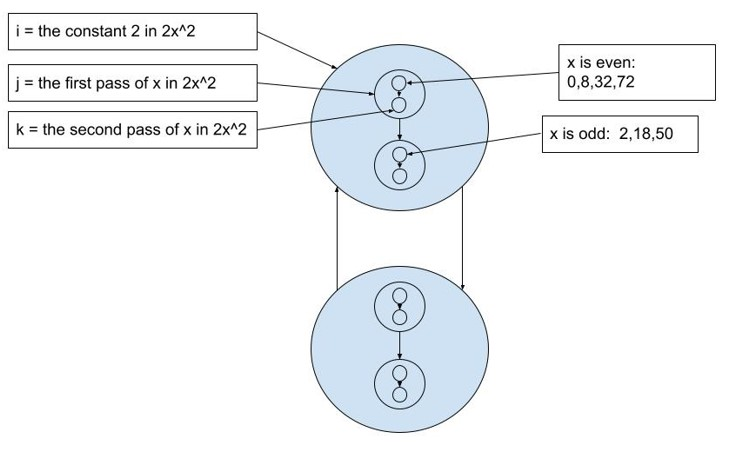
\includegraphics[width=\linewidth]{0205IdealAlgorithm.jpg}
  \caption{The algorithm described visually, $2Decider<2x^2>$.}
  \label{fig:0205IdealAlgorithm}
\end{figure}

\section{Negative Monomials}

Representing negative numbers can be thought of discretely. Below is a representation of negative numbers.

$\\ $

Addition of two negative deciders gives a negative decider.

$Decider<-x> + Decider<-x>$

$ = Decider<-x-x>$

$ = Decider<-2x>$

\begin{figure}[H]
  \centering
  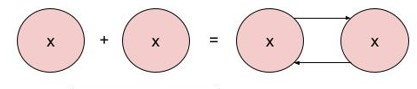
\includegraphics[scale=1]{0207Addition.jpg}
  \caption{Addition.}
  \label{fig:0207Addition}
\end{figure}

$\\ $

Cancellation of a positive and negative decider of such that it is the additive inverse, or 0.

$\\ $

$Decider<x> + Decider<-x>$

$ = Decider<x-x>$

$ = Decider<0>$

\begin{figure}[H]
  \centering
  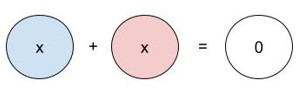
\includegraphics[scale=1]{0206Cancellation.jpg}
  \caption{Cancellation law.}
  \label{fig:0206Cancellation}
\end{figure}

$\\ $

Multiplication of two negative deciders gives a positive decider.

$\\ $

$Decider<-x> * Decider<-x>$

$ = Decider<-x*-x>$

$ = Decider<x^2>$

\begin{figure}[H]
  \centering
  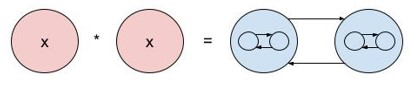
\includegraphics[scale=1]{0208Multiplication.jpg}
  \caption{Multiplication.}
  \label{fig:0208Multiplication}
\end{figure}

$\\ $

Multiplication of a negative decider with its multiplicative inverse gives a its identity, or 1.

$\\ $

$Decider<x^{-1}> * Decider<x>$

$ = Decider<x^{-1}*x>$

$ = Decider<1>$

\begin{figure}[H]
  \centering
  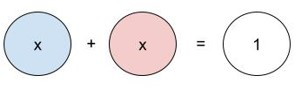
\includegraphics[scale=1]{0209MultiplicativeInverse.jpg}
  \caption{Multiplicative Inverse.}
  \label{fig:0209MultiplicativeInverse}
\end{figure}

\section{Pi}

Representing the constant pi, $\pi$, in the language of polynomials using the Leibniz formula $\pi/4 = 1 - 1/2 + 1/5 -1/7 + 1/9 + \cdots = \sum_{k=0}^{\infty} \frac{(-1)^k}{2k+1}$

$\\ $

\begin{figure}[H]
  \centering
  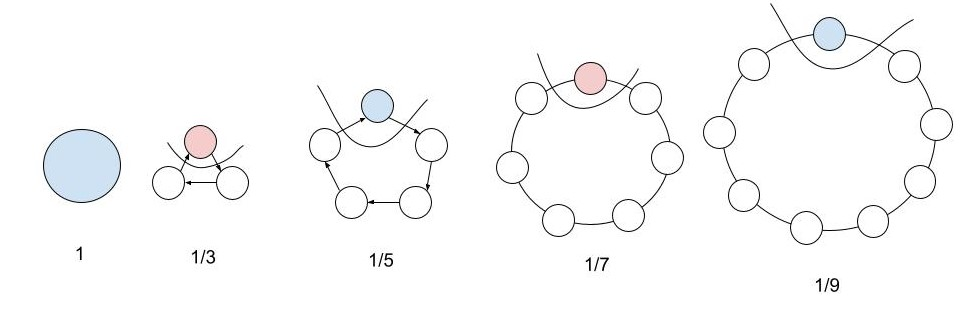
\includegraphics[width=\linewidth]{0210Pi.jpg}
  \caption{Pi under the Leibniz formula to illustrate choosing one state in a decision function of a term decider.}
  \label{fig:0210Pi}
\end{figure}

\section{Analysis of Fibonacci}

A Fibonacci sequence is a sequence of typically seen as the following, ${1,1,2,3,5,8,13,21,\cdots}$. The general formula for this sequence is:

$\\ $

$a_n = a_{n-1} + a_{n-2}$ given $a_0$ and $a_1$

$\\ $

From the example above, we see that f(1) = 1 and f(2) = 2. If we add f(1) and f(2) together we get f(3) = 3 and so on and so forth. The algorithm below will be used to collect data to be analyzed to find a general pattern:

$\\ $

\begin{algorithmic}[1]
\Procedure{Fibonacci}{$n$}
\If {$n = 1$}
	\Return 0
\EndIf
\State $y\gets 1$
\State $y_1\gets 1$
\State $y_2\gets 2$
\For $i = 1\ to\ n-1$
	\State $y\gets y_1 + y_2$
	\State $y_1\gets y_1$
	\State $y_2\gets y$
\EndFor

\Return y
\EndProcedure
\end{algorithmic}

$\\ $

The data collected is organized into input, its parity, output, and its parity. First, the input and its parity value is analyzed in the following:

$\\ $

\begin{figure}[H]
  \centering
  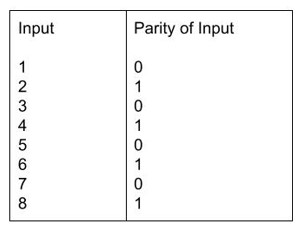
\includegraphics[scale=1]{0211Fibonacci.jpg}
  \caption{The input and the parity of the input of Fibonacci.}
  \label{fig:0211Fibonacci}
\end{figure}

The parity alternates between 0 and 1 which doesn't mean much on its own. Collecting data from the output of the sequence function gives the following:

\begin{figure}[H]
  \centering
  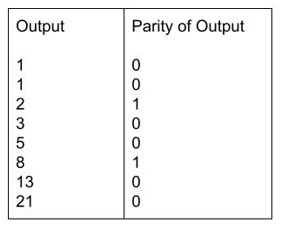
\includegraphics[scale=1]{0212Fibonacci.jpg}
  \caption{The output and the parity of the output of Fibonacci.}
  \label{fig:0212Fibonacci}
\end{figure}

On analysis, it can be seen that there are two patterns mapped out - one from input values 1, 2, and 3 (called {123}) and one from input values 4, 5, and 6 (called {456}). Laying these findings flat on a $3 \times 3$ matrix gives the following:

\begin{figure}[H]
  \centering
  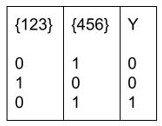
\includegraphics[scale=1]{0213Fibonacci.jpg}
  \caption{The output Y is the output parity.}
  \label{fig:0213Fibonacci}
\end{figure}

There are two matrices that form from analysis of the parity of the input and output. Using the technique to develop an algorithm for the $Decider<2x^2>$ it can be concluded that there are three finishing states for each matrix giving a total of six different finishing states.

\section{Modeling Deciders of Fibonacci}

There exists a mapping between the determinants of the Fibonacci sequence to each state of the Fibonacci sequence. On analyzing the parity of the input of {123}, {456} and the output of the fibonacci sequence, two matrices emerge. Label the input {123} as $E_1$, the input of {456} as $E_2$, and the output of the Fibonacci sequence as $E_3$.

$\\ $

$\begin{array}{ccc}
E_1 & E_2 & E_3\\
0 & 1 & 0\\
1 & 0 & 1\\
0 & 1 & 1\\
\end{array}$

$\\ $

There are six permutations pivoting by the row of the matrices. Three of them have a determinant of -1 and the other three have a determinant 1. The three matrices that have the determinant of -1 are as follows.

$\\ $

$M_1 = \begin{array}{ccc}
E_1 & E_2 & E_3\\
0 & 1 & 0\\
1 & 0 & 1\\
0 & 1 & 1\\
\end{array}$

$\\ $

$M_2 = \begin{array}{ccc}
E_1 & E_2 & E_3\\
1 & 0 & 1\\
0 & 1 & 1\\
0 & 1 & 0\\
\end{array}$

$\\ $

$M_3 = \begin{array}{ccc}
E_1 & E_2 & E_3\\
0 & 1 & 1\\
0 & 1 & 0\\
1 & 0 & 1\\
\end{array}$

$\\ $

The next three matrices that have a determinant of 1 is as follows.

$\\ $

$M_4 = \begin{array}{ccc}
E_1 & E_2 & E_3\\
0 & 1 & 0\\
0 & 1 & 1\\
1 & 0 & 1\\
\end{array}$

$\\ $

$M_5 = \begin{array}{ccc}
E_1 & E_2 & E_3\\
1 & 0 & 1\\
0 & 1 & 0\\
0 & 1 & 1\\
\end{array}$

$\\ $

$M_6 = \begin{array}{ccc}
E_1 & E_2 & E_3\\
0 & 1 & 1\\
1 & 0 & 1\\
0 & 1 & 0\\
\end{array}$

$\\ $

These matrices above would otherwise be called the modulo inverse in most format because it takes the parity, or modulo, of the input and output.

In order to model the Fibonacci sequence, swap the rows $E_1$ and $E_2$ of $M_1$ resulting in the matrix $N_1$. The determinant of $N_1$ is 1 and the rows still have integrity. The matrices can be turned into a sort of adjacency matrix and mapping the the entries of $E_1$ of $M_1$ and $E_2$ of $N_1$ to the value of the states can be seen as a graph in the following:

$\\ $

$E_1 \equiv -x = y - z$

Determinant of $M_1$ = -1

$\\ $

\begin{figure}[H]
  \centering
  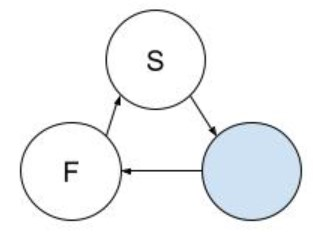
\includegraphics[scale=1]{0214E1.jpg}
  \caption{The determinant of input parity $E_1$ of $M_1$ modeled as a graph visually.}
  \label{fig:0214E1}
\end{figure}


$\\ $

$E_2 \equiv x = -y + z$

Determinant of $N_1$ = 1

$\\ $

\begin{figure}[H]
  \centering
  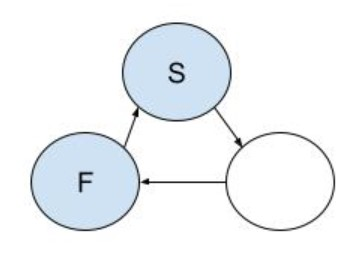
\includegraphics[scale=1]{0215E2.jpg}
  \caption{The determinant of input parity $E_2$ of $N_1$ modeled as a graph visually.}
  \label{fig:0215E2}
\end{figure}

$\\ $

After higher level illustrations and, in addition to the matrices, there are representations of the sequences and, more generally, words that can be formed if a more detailed view of how it operates is needed in linear algebra. A definition below can be traced.

$\\ $

$\textbf{Definition}$. $(S,w) = \lambda\mu w\gamma$.

$\\ $

Set $\lambda$ to a row vector of length 3 filled with ones and $\gamma$ and operate on the matrix, $M_1$ and $N_1$.

$\\ $

$
\lambda\mu_{101} =
\begin{bmatrix}
1 & 1 & 1\\
\end{bmatrix}
\begin{bmatrix}
0 & 1 & 0\\
1 & 0 & 0\\
0 & 1 & 1\\
\end{bmatrix}
=
\begin{bmatrix}
1 & 0 & 1\\
\end{bmatrix}
$

$\\ $

$
\lambda\mu_{011} =
\begin{bmatrix}
1 & 1 & 1\\
\end{bmatrix}
\begin{bmatrix}
1 & 0 & 0\\
0 & 1 & 0\\
1 & 0 & 1\\
\end{bmatrix}
=
\begin{bmatrix}
0 & 1 & 1\\
\end{bmatrix}
$

$\\ $

This result means that there is one even column that permutes between $M_1$ and $N_1$. Now $\gamma$ can be described as the rows being permuted which is the same for both matrices.

$\\ $

$\gamma = 
\begin{bmatrix}
1 \\
1 \\
0 \\
\end{bmatrix}
$

$\\ $ 

Taking the sum of the path of the graph and mapping the state's that represent 0 to -1, the following can be seen.

$\\ $

$E_1 \equiv -x = y - z$

Path of $M_1$ = -1 + 1 - 1 = -1

$\\ $

\begin{figure}[H]
  \centering
  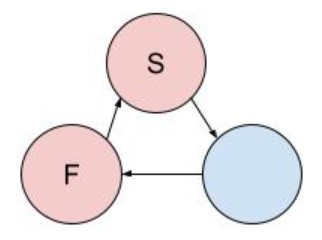
\includegraphics[scale=1]{0216E1.jpg}
  \caption{The sum of input parity $E_1$ of $M_1$ modeled as a graph visually.}
  \label{fig:0216E1}
\end{figure}


$\\ $

$E_2 \equiv x = -y + z$

Path of $N_1$ = 1 - 1 + 1 = 1

$\\ $

\begin{figure}[H]
  \centering
  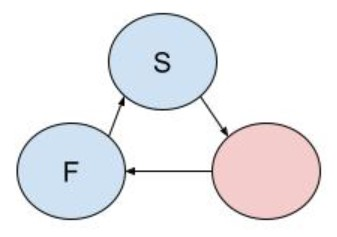
\includegraphics[scale=1]{0217E2.jpg}
  \caption{The sum of input parity $E_2$ of $N_1$ modeled as a graph visually.}
  \label{fig:0217E2}
\end{figure}

$\\ $ 

\section{Redrawing the Fibonacci Sequence}

From our analysis, it can be seen that there are three states that are a minimum to create a Fibonacci sequence. Minimization gives us a monomial generator, ${S_x,S_y,S_z}$. Set the three states to a desired configuration (i.e. $S_y = 0$ and $S_z = 1$ and it will generate the Fibonacci sequence. It can shown that it requires three states minimum to generate the Fibonacci sequence.

$\\ $

Generator

$S_x = S_y + S_z$

$S_y = S_z + S_x$

$S_z = S_x + S_y$

$\\ $

Using the above, dynamic programming can be modeled as a set of generator functions. A visual diagram explains how a set of generator functions form a generator.

$\\ $

\begin{figure}[H]
  \centering
  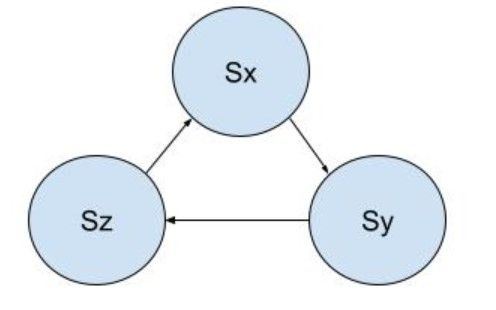
\includegraphics[scale=1]{0218Generator.jpg}
  \caption{The generator for the Fibonacci sequence.}
  \label{fig:0218Generator}
\end{figure}

$\\ $

\begin{algorithmic}[1]
\Procedure{FibonacciGenerator}{$n$}
\State $stateX\gets 0$
\State $stateY\gets 1$
\State $stateZ\gets 1$
\State $cycles\gets 0$
\While {$cycles\leq n+$}
	\State $cycles\gets cycles + 1$
	\If {$cycles > n$}
		\Return $stateX$
	\EndIf
	\State $stateX = stateY + stateZ$
	\State $cycles\gets cycles + 1$
	\If {$cycles > n$}
		\Return $stateY$
	\EndIf
	\State $stateY = stateZ + stateX$
	\State $cycles\gets cycles + 1$
	\If {$cycles > n$}
		\Return $stateZ$
	\EndIf
	\State $stateZ = stateX + stateY$
\EndWhile

\Return $stateX$
\EndProcedure
\end{algorithmic}

$\\ $

\section{The Fibonacci Decider}

Given the two deciders we found using the determinant and the sum of the path by the mapping of the determinants, it is shown that six decision functions and a minimum of six input values are required to decide if a sequence is a type of Fibonacci sequence. In order to create this decider, a composition operator is used on $M_1$ and $N_1$ to merge them together because the sum of the determinant cancels each other. All decision functions must evaluate to true in order for the sequence to be a valid Fibonacci sequence. The following is one possible set of permutations available to form a group of decision functions with the deciders.

$\\ $

$\textit{Example 2.11.1}$. Decider with Decision Functions for $\{123\}$

$x_1 = -y_1 + z_1$

$-x_1 = y_1 + z_1$

$x_1 = y_1 - z_1$

$\\ $

$\textit{Example 2.11.2}$. Decider with Decision Functions for $\{456\}$

$-x_2 = y_2 + -z_2$

$x_2 = -y_2 -z_2$

$-x_2 = -y_2 + z_2$

$\\ $

Join the finish state of $\{123\}$ to the start state of $\{456\}$ and the start state of $\{456\}$ to the finish state of $\{123\}$ to form the Fibonacci decider $\{123456\}$

$\\ $

$\textit{Example 2.11.3}$. Fibonacci decider $\{123456\}$

$x_1 = -y_1 + z_2 - x_2 +y_2 - z_1$

$-y_1 = z_2 - x_2 +y_2 - z_1 + x_1$

$z_2 = x_2 +y_2 - z_1 + x_1 - y_1$

$x_2 = y_2 - z_1 + x_1 - y_1 + z_2$

$y_2 = z_1 + x_1 - y_1 + z_2 - x_2$

$z_1 = x_1 - y_1 + z_2 - x_2+y_2$


\section{The Fibonacci Picking Function}


On analysis, one decision function in $\{123\}$ has three possible permutations. An example is of the following.

$\\ $

Given $x_1 = -y_1 + z_1$, it has $x_1 + y_1 = z_1$ and $x_1 - z_1= -y_1$.

$\\ $

This means that every decision function in $\{123\}$ has three possible permutations, or $3^2$ possibilities, however, if the configuration is desired to be $M_1$ and $N_1$, then there is only one configuration possible out of $3^2$ by $3^2$ possibilities.

After, it can be shown that by applying the picking function, $p_f$, to the Fibonacci decider, the probability is equivalent to $1/n^{k}$.

Each decider has three representations giving $3^2 = 9$ total for each set. There is only one configuration of $M_1$ and $N_1$ given to imply that the probability is $1/9$. Multiply the probability of picking $M_1$ by the probability of picking $N_1$ to get $1/9^{2}$.

There are 6 deciders with 6 permutations each and giving $6^2 = 36$ permutations. 

The probability is then:

$\\ $

$1/3^2 * 1/3^2 \leq 1/6^2$

$\\ $

$\equiv p_f(\{123\})*p_f(\{456\}) \leq 1/n^{k}$ where k = 2

$\\ $

By definition this is called the one way function.

This shows that the relation between $M_1\ of\ \{123\}$ and $N_1\ of\ \{456\}$ and the formation of $\{123456\}$.

This shows a concrete example of the picking function which is a type of one way function.
